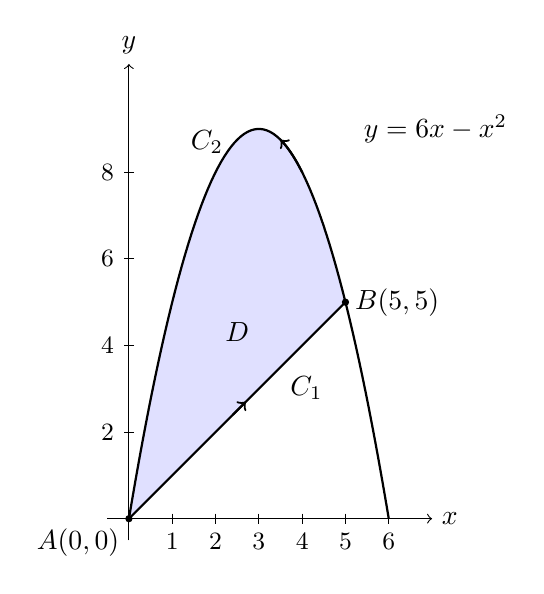
\begin{tikzpicture}[scale=0.55]
    % Ejes
    \draw[->] (-0.5, 0) -- (7, 0) node[right] {$x$};
    \draw[->] (0, -0.5) -- (0, 10.5) node[above] {$y$};

    % Región sombreada entre la recta y la parábola en [0,5]
    \fill[blue!12, domain=0:5, samples=80] 
        plot ({\x}, {6*\x - \x*\x}) -- (5,5) -- (0,0) -- cycle;

    % Parábola y = 6x - x^2  (tramo C_2, orientado de B a A)
    \draw[thick, domain=0:6, samples=80] plot ({\x}, {6*\x - \x*\x});
    % Flecha de orientación sobre la parábola (de derecha a izquierda)
    \draw[thick, ->] plot [domain=4:3.5, samples=20] ({\x}, {6*\x - \x*\x});

    % Recta y = x  (tramo C_1, orientado de A a B)
    \draw[thick] (0,0) -- (5,5);
    \draw[thick, ->] (2.4, 2.4) -- (2.7, 2.7);

    % Puntos
    \filldraw (0,0) circle (2pt) node[below left] {$A(0,0)$};
    \filldraw (5,5) circle (2pt) node[right] {$B(5,5)$};

    % Etiquetas
    \node at (2.5, 4.3) {$D$};
    \node[below right] at (3.5, 3.5) {$C_1$};
    \node[above] at (1.8, 8.2) {$C_2$};
    \node[right] at (5.2, 9) {$y = 6x - x^2$};
    \node[right] at (5, 5) {};

    % Marcas en los ejes
    \foreach \x in {1,2,3,4,5,6}
        \draw (\x, 0.12) -- (\x, -0.12) node[below] {\small\x};
    \foreach \y in {2,4,6,8}
        \draw (0.12, \y) -- (-0.12, \y) node[left] {\small\y};
\end{tikzpicture}